
%% Beginning of file 'sample63.tex'
%%
%% Modified 2019 June
%%
%% This is a sample manuscript marked up using the
%% AASTeX v6.3 LaTeX 2e macros.
%%
%% AASTeX is now based on Alexey Vikhlinin's emulateapj.cls 
%% (Copyright 2000-2015).  See the classfile for details.

%% AASTeX requires revtex4-1.cls (http://publish.aps.org/revtex4/) and
%% other external packages (latexsym, graphicx, amssymb, longtable, and epsf).
%% All of these external packages should already be present in the modern TeX 
%% distributions.  If not they can also be obtained at www.ctan.org.

%% The first piece of markup in an AASTeX v6.x document is the \documentclass
%% command. LaTeX will ignore any data that comes before this command. The 
%% documentclass can take an optional argument to modify the output style.
%% The command below calls the preprint style which will produce a tightly 
%% typeset, one-column, single-spaced document.  It is the default and thus
%% does not need to be explicitly stated.
%%
%%
%% using aastex version 6.3
\documentclass{aastex63}

%% The default is a single spaced, 10 point font, single spaced article.
%% There are five other style options available via an optional argument. 
%% They can be invoked like this:
%%
%% \documentclass[arguments]{aastex63}
%% 
%% where the layout options are:
%%
%%  twocolumn   : two text columns, 10 point font, single spaced article.
%%                This is the most compact and represent the final published
%%                derived PDF copy of the accepted manuscript from the publisher
%%  manuscript  : one text column, 12 point font, double spaced article.
%%  preprint    : one text column, 12 point font, single spaced article.  
%%  preprint2   : two text columns, 12 point font, single spaced article.
%%  modern      : a stylish, single text column, 12 point font, article with
%% 		  wider left and right margins. This uses the Daniel
%% 		  Foreman-Mackey and David Hogg design.
%%  RNAAS       : Preferred style for Research Notes which are by design 
%%                lacking an abstract and brief. DO NOT use \begin{abstract}
%%                and \end{abstract} with this style.
%%
%% Note that you can submit to the AAS Journals in any of these 6 styles.
%%
%% There are other optional arguments one can invoke to allow other stylistic
%% actions. The available options are:
%%
%%   astrosymb    : Loads Astrosymb font and define \astrocommands. 
%%   tighten      : Makes baselineskip slightly smaller, only works with 
%%                  the twocolumn substyle.
%%   times        : uses times font instead of the default
%%   linenumbers  : turn on lineno package.
%%   trackchanges : required to see the revision mark up and print its output
%%   longauthor   : Do not use the more compressed footnote style (default) for 
%%                  the author/collaboration/affiliations. Instead print all
%%                  affiliation information after each name. Creates a much 
%%                  longer author list but may be desirable for short 
%%                  author papers.
%% twocolappendix : make 2 column appendix.
%%   anonymous    : Do not show the authors, affiliations and acknowledgments 
%%                  for dual anonymous review.
%%
%% these can be used in any combination, e.g.
%%
%% \documentclass[twocolumn,linenumbers,trackchanges]{aastex63}
%%
%% AASTeX v6.* now includes \hyperref support. While we have built in specific
%% defaults into the classfile you can manually override them with the
%% \hypersetup command. For example,
%%
%% \hypersetup{linkcolor=red,citecolor=green,filecolor=cyan,urlcolor=magenta}
%%
%% will change the color of the internal links to red, the links to the
%% bibliography to green, the file links to cyan, and the external links to
%% magenta. Additional information on \hyperref options can be found here:
%% https://www.tug.org/applications/hyperref/manual.html#x1-40003
%%
%% Note that in v6.3 "bookmarks" has been changed to "true" in hyperref
%% to improve the accessibility of the compiled pdf file.
%%
%% If you want to create your own macros, you can do so
%% using \newcommand. Your macros should appear before
%% the \begin{document} command.
%%
\newcommand{\vdag}{(v)^\dagger}
\newcommand\aastex{AAS\TeX}
\newcommand\latex{La\TeX}



\usepackage{color}

\usepackage{times}
\newcommand{\sqcm}{cm$^{-2}$}
\newcommand{\alphaox}{$\alpha_{OX}$}
\newcommand{\Gammaxray}{$\Gamma$}

\newcommand{\fek}{Fe~K$\alpha$}
\newcommand{\xmm}{{\em XMM-Newton}}
\newcommand{\nustar}{{\em NuSTAR}}
\newcommand{\chandra}{{\em Chandra}}
\newcommand{\swift}{{\em Swift}}
\newcommand{\suzaku}{{\em Suzaku}}
\newcommand{\sax}{{\em BeppoSAX}}
\usepackage[space]{grffile}
\usepackage[]{amsmath}
\usepackage{amssymb}
\usepackage[normalem]{ulem}
\usepackage{natbib}
%\usepackage{hyperref}
\usepackage{comment}
\bibpunct{(}{)}{;}{a}{}{,}
%\usepackage{pdflscape}	% Landscape pages
\usepackage{amsmath} % or simply amstext
\newcommand{\angstrom}{\text{\normalfont\AA}}
\usepackage{url}
\texorpdfstring
%\usepackage{showframe}









%% Reintroduced the \received and \accepted commands from AASTeX v5.2
\received{November  X, 2019}
\revised{November  X, 2019}
\accepted{\today}
%% Command to document which AAS Journal the manuscript was submitted to.
%% Adds "Submitted to " the argument.
\submitjournal{APJ}

%% For manuscript that include authors in collaborations, AASTeX v6.3
%% builds on the \collaboration command to allow greater freedom to 
%% keep the traditional author+affiliation information but only show
%% subsets. The \collaboration command now must appear AFTER the group
%% of authors in the collaboration and it takes TWO arguments. The last
%% is still the collaboration identifier. The text given in this
%% argument is what will be shown in the manuscript. The first argument
%% is the number of author above the \collaboration command to show with
%% the collaboration text. If there are authors that are not part of any
%% collaboration the \nocollaboration command is used. This command takes
%% one argument which is also the number of authors above to show. A
%% dashed line is shown to indicate no collaboration. This example manuscript
%% shows how these commands work to display specific set of authors 
%% on the front page.
%%
%% For manuscript without any need to use \collaboration the 
%% \AuthorCollaborationLimit command from v6.2 can still be used to 
%% show a subset of authors.
%
%\AuthorCollaborationLimit=2
%
%% will only show Schwarz & Muench on the front page of the manuscript
%% (assuming the \collaboration and \nocollaboration commands are
%% commented out).
%%
%% Note that all of the author will be shown in the published article.
%% This feature is meant to be used prior to acceptance to make the
%% front end of a long author article more manageable. Please do not use
%% this functionality for manuscripts with less than 20 authors. Conversely,
%% please do use this when the number of authors exceeds 40.
%%
%% Use \allauthors at the manuscript end to show the full author list.
%% This command should only be used with \AuthorCollaborationLimit is used.

%% The following command can be used to set the latex table counters.  It
%% is needed in this document because it uses a mix of latex tabular and
%% AASTeX deluxetables.  In general it should not be needed.
%\setcounter{table}{1}

%%%%%%%%%%%%%%%%%%%%%%%%%%%%%%%%%%%%%%%%%%%%%%%%%%%%%%%%%%%%%%%%%%%%%%%%%%%%%%%%
%%
%% The following section outlines numerous optional output that
%% can be displayed in the front matter or as running meta-data.
%%
%% If you wish, you may supply running head information, although
%% this information may be modified by the editorial offices.
\shorttitle{Mrk 1018}
\shortauthors{Bing Lyu et al.}
%%
%% You can add a light gray and diagonal water-mark to the first page 
%% with this command:
%% \watermark{text}
%% where "text", e.g. DRAFT, is the text to appear.  If the text is 
%% long you can control the water-mark size with:
%% \setwatermarkfontsize{dimension}
%% where dimension is any recognized LaTeX dimension, e.g. pt, in, etc.
%%
%%%%%%%%%%%%%%%%%%%%%%%%%%%%%%%%%%%%%%%%%%%%%%%%%%%%%%%%%%%%%%%%%%%%%%%%%%%%%%%%
\graphicspath{{./}{figures/}}
%% This is the end of the preamble.  Indicate the beginning of the
%% manuscript itself with \begin{document}.

\begin{document}

\title{Long term multi-wavelength evolution of Changing-Look AGN: Mrk~1018}

%% LaTeX will automatically break titles if they run longer than
%% one line. However, you may use \\ to force a line break if
%% you desire. In v6.3 you can include a footnote in the title.

%% A significant change from earlier AASTEX versions is in the structure for 
%% calling author and affiliations. The change was necessary to implement 
%% auto-indexing of affiliations which prior was a manual process that could 
%% easily be tedious in large author manuscripts.
%%
%% The \author command is the same as before except it now takes an optional
%% argument which is the 16 digit ORCID. The syntax is:
%% \author[xxxx-xxxx-xxxx-xxxx]{Author Name}
%%
%% This will hyperlink the author name to the author's ORCID page. Note that
%% during compilation, LaTeX will do some limited checking of the format of
%% the ID to make sure it is valid. If the "orcid-ID.png" image file is 
%% present or in the LaTeX pathway, the OrcID icon will appear next to
%% the authors name.
%%
%% Use \affiliation for affiliation information. The old \affil is now aliased
%% to \affiliation. AASTeX v6.3 will automatically index these in the header.
%% When a duplicate is found its index will be the same as its previous entry.
%%
%% Note that \altaffilmark and \altaffiltext have been removed and thus 
%% can not be used to document secondary affiliations. If they are used latex
%% will issue a specific error message and quit. Please use multiple 
%% \affiliation calls for to document more than one affiliation.
%%
%% The new \altaffiliation can be used to indicate some secondary information
%% such as fellowships. This command produces a non-numeric footnote that is
%% set away from the numeric \affiliation footnotes.  NOTE that if an
%% \altaffiliation command is used it must come BEFORE the \affiliation call,
%% right after the \author command, in order to place the footnotes in
%% the proper location.
%%
%% Use \email to set provide email addresses. Each \email will appear on its
%% own line so you can put multiple email address in one \email call. A new
%% \correspondingauthor command is available in V6.3 to identify the
%% corresponding author of the manuscript. It is the author's responsibility
%% to make sure this name is also in the author list.
%%
%% While authors can be grouped inside the same \author and \affiliation
%% commands it is better to have a single author for each. This allows for
%% one to exploit all the new benefits and should make book-keeping easier.
%%
%% If done correctly the peer review system will be able to
%% automatically put the author and affiliation information from the manuscript
%% and save the corresponding author the trouble of entering it by hand.


\author{To be determind}

\begin{comment}
\author[0000-0001-8879-368X]{Bing Lyu}
\affiliation{Huazhong University of Science and Technology \\
School of Physics, 1037 Luoyu Road \\
Wuhan, 430074, China \\}
%\affil{Shanghai Astronomical Observatory\\ CAS, Nandan Road 80 \\ Shanghai, 200030, China}
%\nocollaboration
\author[0000-0002-5385-9586]{Zhen Yan}
\affil{Shanghai Astronomical Observatory\\
CAS, Nandan Road 80 \\
Shanghai, 200030, China}



\author[0000-0002-3844-9677]{Wenfei Yu}
\affiliation{Shanghai Astronomical Observatory\\
CAS, Nandan Road 80 \\
Shanghai, 200030, China}
%\collaboration{(AAS Journals Data Scientists collaboration)}

\author[0000-0003-4773-4987]{Qingwen Wu}
\affiliation{Huazhong University of Science and Technology \\
School of Physics, 1037 Luoyu Road \\
Wuhan, 430074, China \\}

%\correspondingauthor{Qingwen Wu}
%\email{qwwu@hust.edu.cn}
\end{comment}
%\nocollaboration



%% Note that the \and command from previous versions of AASTeX is now
%% depreciated in this version as it is no longer necessary. AASTeX 
%% automatically takes care of all commas and "and"s between authors names.

%% AASTeX 6.3 has the new \collaboration and \nocollaboration commands to
%% provide the collaboration status of a group of authors. These commands 
%% can be used either before or after the list of corresponding authors. The
%% argument for \collaboration is the collaboration identifier. Authors are
%% encouraged to surround collaboration identifiers with ()s. The 
%% \nocollaboration command takes no argument and exists to indicate that
%% the nearby authors are not part of surrounding collaborations.

%% Mark off the abstract in the ``abstract'' environment. 
\begin{abstract}
We present multi-wavelength and long-term evolution of Changing-look AGN, Mrk~1018, especially during its fading phase, which shows rapid variability in X-ray and optical band. While Mrk~1018 shows strong correlation between UVOT and X-ray band, the flux in UVOT varies more than that in X-ray as a whole but reverses during type transition period within short timescale. The type transition timescale for Mrk~1018 is around 2 years or less, while we find the minimum timescale for variability can be as short as $\sim$ 100 days. The photon index($\Gamma$) indicating the hardness in X-ray and $\alpha_{OX}$ representing the relative strength of ultraviolet and X-ray, which are good probe of corona and accretion disk, both appear as "V-shape" when compared to luminosity, even though there is a wide gap. We find $\alpha_{OX}$ rather than $\Gamma$ is a better symbol of the type of AGN. However, only weak variability appears in the radio band, makes it hard to understand the mechanism of radio emission.  
\end{abstract}
%% Keywords should appear after the \end{abstract} command. 
%% See the online documentation for the full list of available subject
%% keywords and the rules for their use.
\keywords{AGN: Changing-look -- AGN: individual (Mrk~1018)}



%% From the front matter, we move on to the body of the paper.
%% Sections are demarcated by \section and \subsection, respectively.
%% Observe the use of the LaTeX \label
%% command after the \subsection to give a symbolic KEY to the
%% subsection for cross-referencing in a \ref command.
%% You can use LaTeX's \ref and \label commands to keep track of
%% cross-references to sections, equations, tables, and figures.
%% That way, if you change the order of any elements, LaTeX will
%% automatically renumber them.
%%
%% We recommend that authors also use the natbib \citep
%% and \citet commands to identify citations.  The citations are
%% tied to the reference list via symbolic KEYs. The KEY corresponds
%% to the KEY in the \bibitem in the reference list below. 

\section{Introduction}\label{sec:intro} 
Unified active galactic nucleus(AGN) scheme can be described as a phenomenon that different AGN types are determined by the effect of different inclination to line of sight, see \citet{1993ARA&A..31..473A}. Under this scheme, Seyferts were first classified as Type I or II, depending on the emission lines shown by their spectra. Type I(S1) AGNs, show broad lines, allowed lines and narrower forbidden lines, could be face-on to observer, while type II(S2) AGNs show only both permitted and forbidden narrow lines, which could be edge-on and blocked by surrounding torus. Subclasses(e.g. Seyfert 1.5, 1.8 and 1.9) were introduced by \citet{1976MNRAS.176P..61O,1981ApJ...249..462O} based on the relative weaker ratio of broad-line components to the narrow-line component. For type 1.9, only $H\alpha$ line shows in the broad-line components. 

Mrk~1018 at z=0.042436 is known to be a changing-look AGN, which has undergone a full cycle with twice type transition. \citet{1986ApJ...311..135C} reported that the type of Mrk~1018 transited from S1.9 to S1 between 1979 and 1984. \citet{2016A&A...593L...8M} reported that Mrk~1018 returned to S1.9 between 2013 and 2015 after 30 years as a S1 \citep[see also][]{2017A&A...607L...9K}. A tidal eruption event could not account for the Mrk 1018's change. As reported in \citet{2016A&A...593L...9H}, the optical continuum brightness and X-ray flux drops by a factor of $\sim$ 17 and $\sim 8$, respectively, in 2010$\sim$2016 and an explanation of obscuration event is ruled out. Since no intrinsic absorption in the X-ray spectrum is detected, it comes  to the conclusion that change of type is consistent with declining accretion rate. \citet{2017A&A...607L...9K} reported the outburst of Mrk~1018 in October 2016 with the brightening by a factor of 1.9 at least to February 2017. Far-UV continuum flux also increased by a factor of 1.5 in around one year during the outburst. It seems that radiation of corona and accretion disk comes from near region. We notice that Mrk~1018 has also experienced the re-brightening during the types transition period simultaneously in X-ray and UVOT band by a factor of $\sim3$ and $\sim1.3$, respectively, between 2013 Mar and 2013 Jun. With broad-band spectrum fitting in two states, \citet{2018MNRAS.480.3898N} suggests the drop of soft X-ray excess contributing most ionizing photons causes the disappearance of Broad Line Region(BLR) then the type transition. \citet{2018ApJ...861...51K} models the broad-line component with a recoiled super-massive black hole scenario with a $\sim$29 years orbital period and predicts that if the type transition repeats as past, it would occur again in mid-2020s. Before that, what the mechanism for such short-timescale light curve variability for AGN and type transition is remains unclear. We use the photon index ($\Gamma$, hereafter) in X-ray and \alphaox ~ as probe to trace the relationship between corona and accretion disk during the type transition of Mrk~1018. Here we define \alphaox as :
\begin{equation}
\alpha_{OX}  = - \frac{log(\lambda F_{2500 \angstrom}/\nu F_{2keV})}{log(\nu_{ 2500 \angstrom }/\nu_{2keV})}+1
\end{equation}
The flux is converted by magnitude in the UVW1 filter with central wavelength {2600{$\angstrom$}} and full-width at half max of $\sim 683\angstrom$ \citep{2008MNRAS.383..627P} to estimate $\lambda F_{2500 \angstrom}$.  

This paper is structured as follows: In Sect. \ref{sec:data}, we describe the observations and data reduction. In Sect. ~\ref{sec:result}, we present multi-wavelength observation result. In last Sect. ~\ref{sec:discussion}, we discuss possible explanations for the observation of Mrk~1018. Hereafter, we adopt $H_0$=70 km $s^{-1} Mpc^{-1}$, $\Omega_{m}$=0.3, and $\Omega_{\Lambda}=0.7 $ as cosmological parameters, and the latest Black Hole(BH) mass measurement $\log(M_{BH}/M_{\odot})=7.84$ \citep{2017MNRAS.472.3492E,2018MNRAS.480.3898N}. 
%\clearpage


\section{Data Analysis}\label{sec:data}
\subsection{X-ray}
We analyse archival \swift, \xmm, \chandra~and \nustar~data in 2005 $\sim$ 2018. All 2-10~keV fluxes are corrected for Galactic absorption with cflux model in Xspec v12.10.1f \citep{1996ASPC..101...17A}, where its absorption by Galactic neutral hydrogen, nH, was fixed at 0.0243 $\times 10^{22} cm^{-2}$\citep[see ][]{2016A&A...593L...9H}. All best fit parameters include photon index($\Gamma$), flux in 2-10~keV($F_{2-10~keV}$) after the Galactic absorption correction, etc, and observation information are listed in Table.~\ref{tab:table1}.


\subsubsection{\swift/XRT}
The X-Ray Telescope (XRT) on board the Swift satellite has the most frequent long term X-ray observation of Mrk~1018. We analysis the archive data with xrtpipeline\footnote{\url{http://swift.asdc.asi.it}} and fit the spectrum of Mrk~1018 in 0.5-10~keV range based on a simple absorbed power-law model for all data.  The source region is a 47-arcsec-radius circle at the center of AGN as suggested in \citet{2009MNRAS.397.1177E}. When counts of photons is less than 100, we use C-stat method to fit the model without grouping counts bins. Otherwise, the spectrum is grouped by minimum of 20 counts per bin. 


\subsubsection{\chandra}
We use ciao 4.10\footnote{\url{http://cxc.harvard.edu/ciao/threads/index.html}} to analysis the 6 Chandra observations released in archive data. All data is grouped by minimum of 20 counts per bin and fitted in 0.5-10~keV range by a absorbed power-law plus gaussian component, except for the observation in 2010, for which pile-up effects should be carefully taken into account. The source and background regions selection follow \citet{2017ApJ...840...11L}, which takes care of accounting for the effects of pile-up with a JDPILEUP component and get the  $\Gamma =1.97_{+0.04}^{-0.03}$. It's similar to our result $\Gamma =2.02\pm{0.03}$ when we consider the pile-up effects. The correction for pile-up effects will make the spectrum softer. \citet{2016A&A...593L...9H} excluded the brightest 9 pixels to avoid pile-up effects and get a lower $\Gamma =1.68\pm0.04$ determined from 4-8 keV range spectrum. \citet{2017A&A...607L...9K} ignored the pile-up effects and get a similar $\Gamma =1.7\pm0.03$ fitted in 0.5-8 keV. The fitting range selection will also influence the parameter $\Gamma$. So we adopted values from \citet{2017A&A...607L...9K} for the observation in 2010(MJD 55527).

\subsubsection{\xmm/EPIC-PN}
Only 2 observation data in 2005 and 2008 with XMM-Newton have been released, and we analysis the data with xmmsas-20170719-1539-16.1.0.\footnote{\url{https://www.cosmos.esa.int/web/xmm-newton}}. The spectrum is grouped by minimum of 30 counts per bin and fitted in the 2-10~keV range based on a absorbed power-law model. 

\subsubsection{\nustar}
5 observations with Nustar in archive data are analysised with nupipeline version 0.4.6 within heasoft v6.26.\footnote{\url{https://heasarc.gsfc.nasa.gov/docs/software/lheasoft/}}. The source region is a 50-arcsec-radius circle at the center of AGN, and background is extracted from region off source. The spectrum is grouped by minimum of 30 counts per bin and fitted in the 3-79~keV range based on a absorbed power-law model.


\subsection{Optical/ultraviolet}
\subsubsection{\swift/UVOT}
There are six filters in optical/ultraviolet band of \swift/UVOT: V,B,U,UVW1,UVM2 and UVW2. We use the tool \textit{uvotsource} to do the aperture photometry for all the observations of each filter. The source aperture radius is 5$\arcsec$ and the background is chosen in a blank region with much larger aperture radius. The results of the V and B filters are discarded, because the emission from the host galaxy is dominated in these two bands even in the bright phase \citep{2018MNRAS.480.3898N}. We discard the results of all filters after 2016, since the emission from the nucleus is comparable or less than the host galaxy \citep{2018MNRAS.480.3898N}, see Tab.~\ref{tab:tablealpha_ox} for details. Milky Way extinction correction with \texorpdfstring{E(B$-V$) = 0.024}. mag \footnote{Retrieved via the NASA/IPAC Extragalactic Database (NED): \url{http://ned.ipac.caltech.edu/}} with extinction model from \citet{2007ApJ...663..320F} is adopted.  
%($A_V=$ 0.075 and $R_{V}=3.1$)


\subsection{Radio/VLA}
%\label{subsec:vla}
%\subsubsection{VLA}
We search all the historical VLA observations on Mrk~1018 within the field of view. For data reduction of old VLA data(project AU0020, AB0476, AB0540 and AB0878), we manually flag and calibrate the data, then clean the image following the instruction\footnote{\url{https://casaguides.nrao.edu/index.php/VLA_5_GHz_continuum_survey_of_Seyfert_galaxies}}. For all JVLA data(project 16A-444, 16B-084),  we analysis the data with CASA version 5.3.0\citep{2007ASPC..376..127M}. All calibration are performed using scripted EVLA\_pipeline1.4.2\footnote{\url{https://science.nrao.edu/facilities/vla/data-processing/pipeline/scripted-pipeline}}. Different bands are split into different MS files after pipeline calibration and RFI check. Then the source are imaged using TCLEAN method and flux are estimated via IMFIT task. The flux density uncertainties are calculated as $\sigma_{S}=\sqrt{(rms)^2+(0.05\times S)^2}$, where $5\%$ absolute flux error is taken into account. Radio spetrum index $\alpha$ is estimated following $S_v \propto v^{-\alpha}$. Survey results in FIRST\citep{1994ASPC...61..165B,1995ApJ...450..559B} and Stripe 82\citep{2011AJ....142....3H} from archival papers are also listed in Table.~\ref{tab:tableradio}.

\section{Result}
\label{sec:result}

\subsection{Multi-band light curve}
The decay timescale fitted with a exponential function is $\sim$2000 and $\sim$1000 days for light curve in XRT and UVOT band. 

\begin{figure}
\centering
	% To include a figure from a file named example.*
	% Allowable file formats are eps or ps if compiling using latex
	% or pdf, png, jpg if compiling using pdflatex
	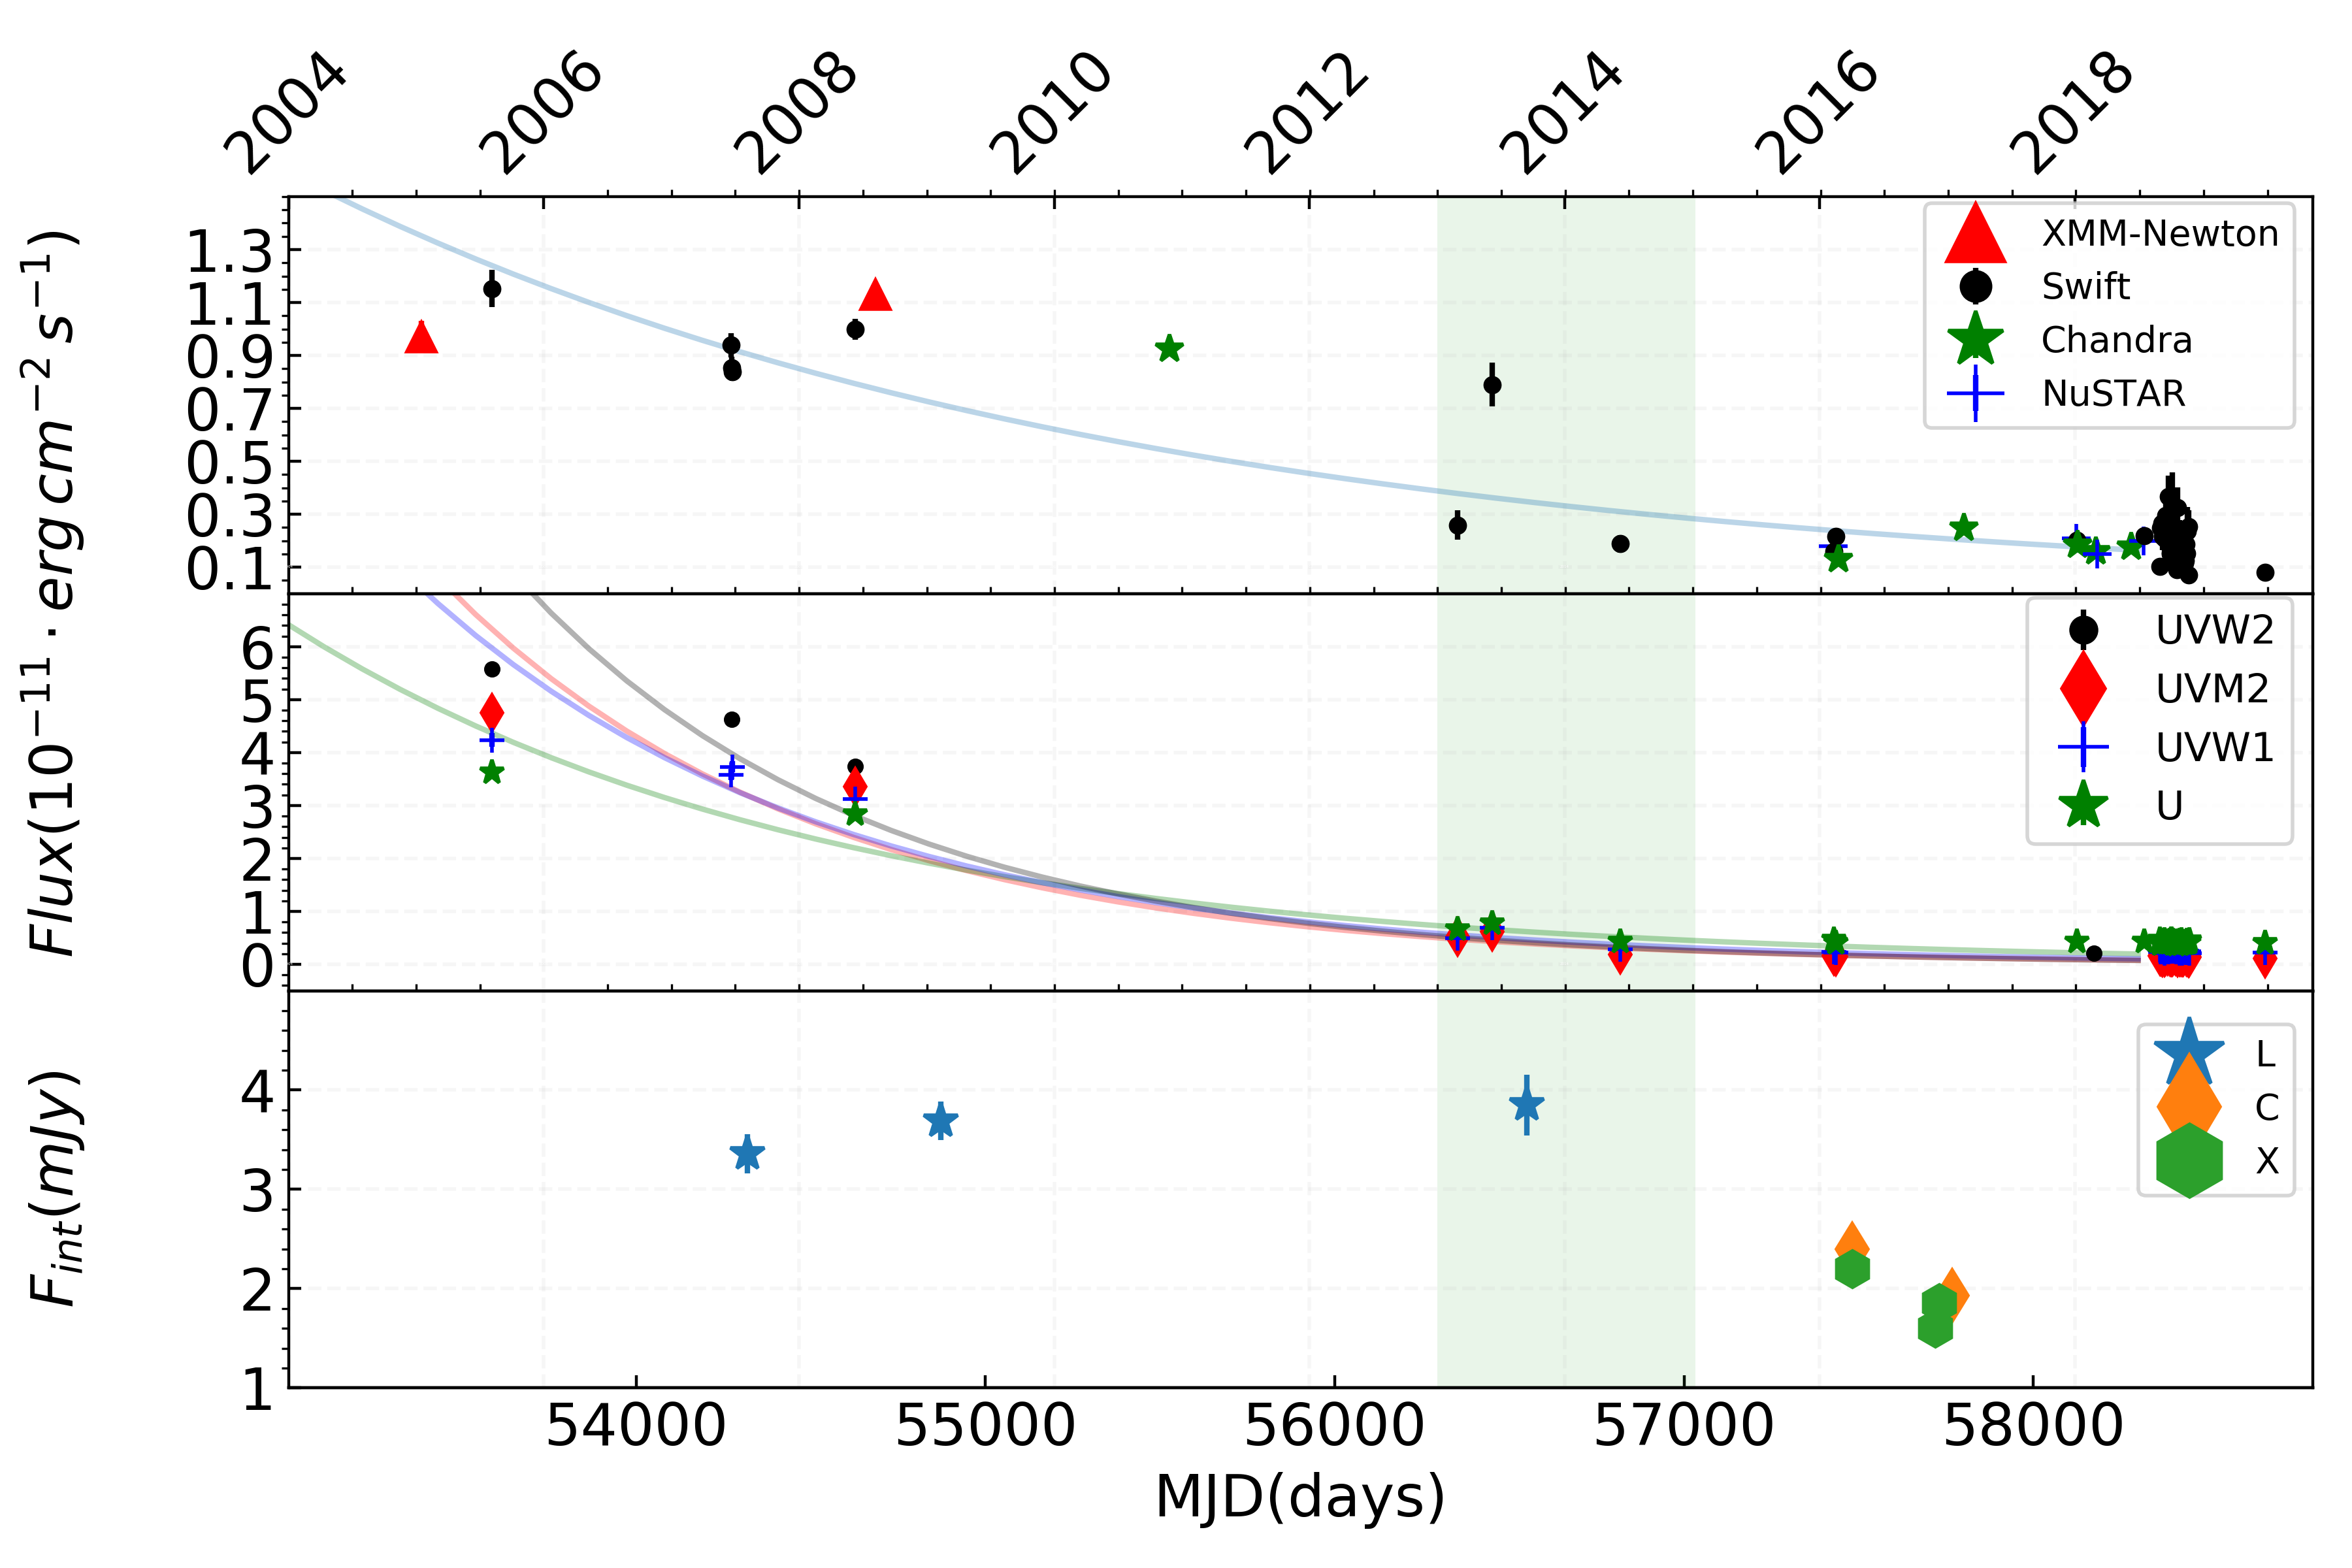
\includegraphics[width=0.8\textwidth]{./pic/subplots-xrt_uvot-radio-second.png}
    \caption{Multi-wavelength light curve of Mrk~1018.}
    \label{fig:multi-lc-secondaxis}
\end{figure}


\subsection{Evolution of photon index(~\texorpdfstring{$\Gamma$}.) and ~\texorpdfstring{$\alpha_{OX}$}.~ with Eddington rate \label{subsec:g-f}}

Based on all X-ray spectrum fit, we show the photon index evolution with flux and Eddington rate, as shown in Fig.~\ref{fig:xrayappendgood-fandg-tmap}. For XRT observations, we only adopt data with 0.7$\le \chi^2_{reduced} \le$1.5. The $\Gamma$ vs Eddington rate diagram shows distinct evolution relationship when $L_{2-10~ keV}/L_{Edd}$ reach the so-called critical Eddington rate around 0.002$\sim$ 0.01. The evolution of spectrum and the dimming of X-ray flux might be caused by the central engine activities as the intrinsic absorption(nH) is consistent with zero. However, we find that it transits in two branches in short timescale(100-800 days) relative to the typical timescale of Super-massive Black Holes(SMBHs). We emphasise that Mrk~1018 increases its flux in X-ray by a factor $\sim3$ from MJD 56352 to 56450, while $\Gamma$ drops from $\sim1.8$ to $\sim1.4$, which appeares in two branches. However, the $\alpha_{OX}$ varies just a little and appears in left branch during the same re-brightening. The $\alpha_{OX}$-Eddington rate diagram is in good agreement with two other changing-look AGNs, see Fig.~\ref{fig:alpha_ox_luv}. 




\subsection{Correlation between X-ray and ultraviolet}
During the fading phase, the X-ray flux shows strong linear correlation with UVOT data. The spearmanr coefficiency between simultaneous flux of xrt and four uvot band(uvm2,u,uvw1,and uvw2) are 0.99, 0.9, 0.86, 0.94, respectively. Both in X-ray and UVOT band, it shows the brightening from MJD 56352 to 56450. We find an outlier in Fig.~\ref{fig:correlation-uvot-xray} since the flux during this period in x-ray and four uvot  band(uvm2,u,uvw1,and uvw2) increases by a factor of $\sim 3.2$ and $\sim 1.2$, $\sim 1.2$, $\sim 1.4$, $\sim 1.5$, respectively. Then the flux fades by a factor of $\sim 4.2$ and $\sim 3.3$, $\sim 1.8$, $\sim 2.5$, $\sim 3$, respectively, from MJD 56450 to 56817. The slopes between log($F_{2-10keV}$) and four band log($\lambda F_{\lambda}$) are 1.7, 1.1, 1.5, 1.8, respectively, after excluding the outlier.


\begin{figure}
\centering
	% To include a figure from a file named example.*
	% Allowable file formats are eps or ps if compiling using latex
	% or pdf, png, jpg if compiling using pdflatex
	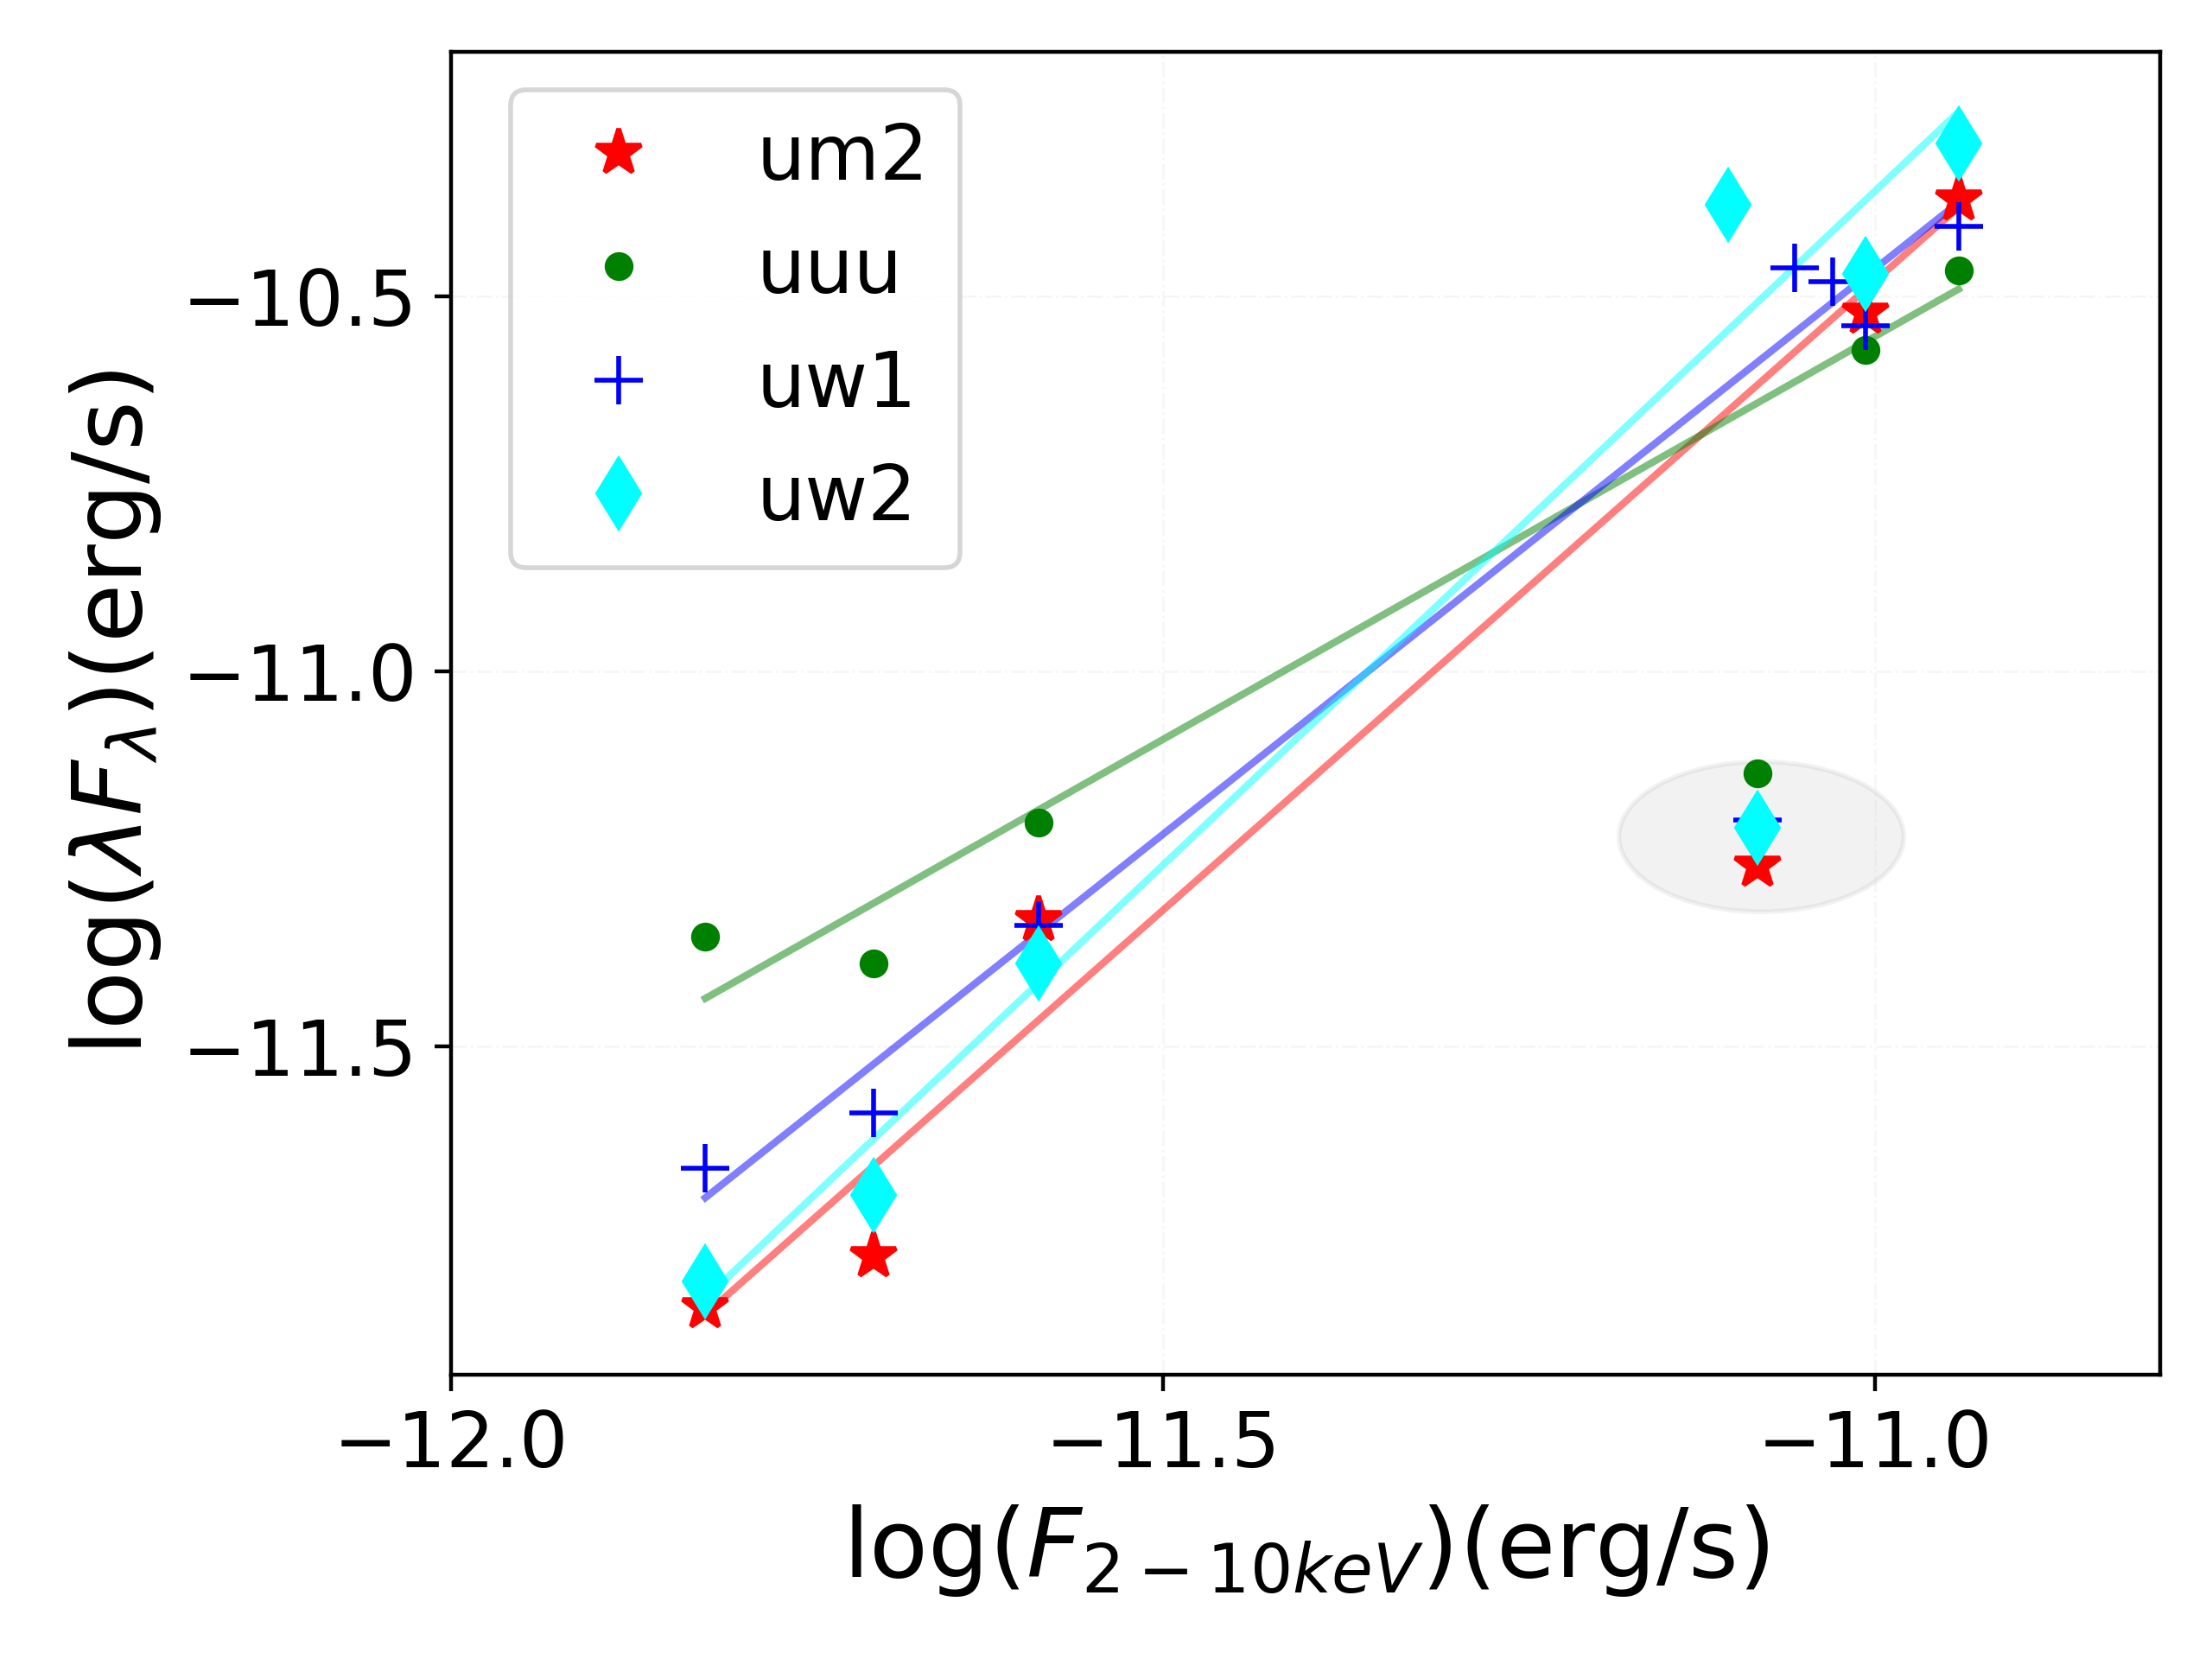
\includegraphics[width=0.9\textwidth]{./pic/uvot_xrt_correlation-fig-without-outlier.png}
    \caption{Correlation of light curve from UVOT and XRT  between 2006 and 2016. Line represent the linear fit without the outlier in circle.}
    \label{fig:correlation-uvot-xray}
\end{figure}








%%%%%%%%%%%%%%%%%%%%%%%%%%%%%
%\subsection{\texorpdfstring{$\alpha_{OX}-L$}. diagram \label{subsec:alpha_ox}}







\subsection{SED between X-ray and ultraviolet}\label{subsec:xray-uvot-sed}
As the flux drops in X-ray and UVOT band, the spectrum also changes, and the temperature of disk declines as well.
\begin{figure}
\centering
	% To include a figure from a file named example.*
	% Allowable file formats are eps or ps if compiling using latex
	% or pdf, png, jpg if compiling using pdflatex
	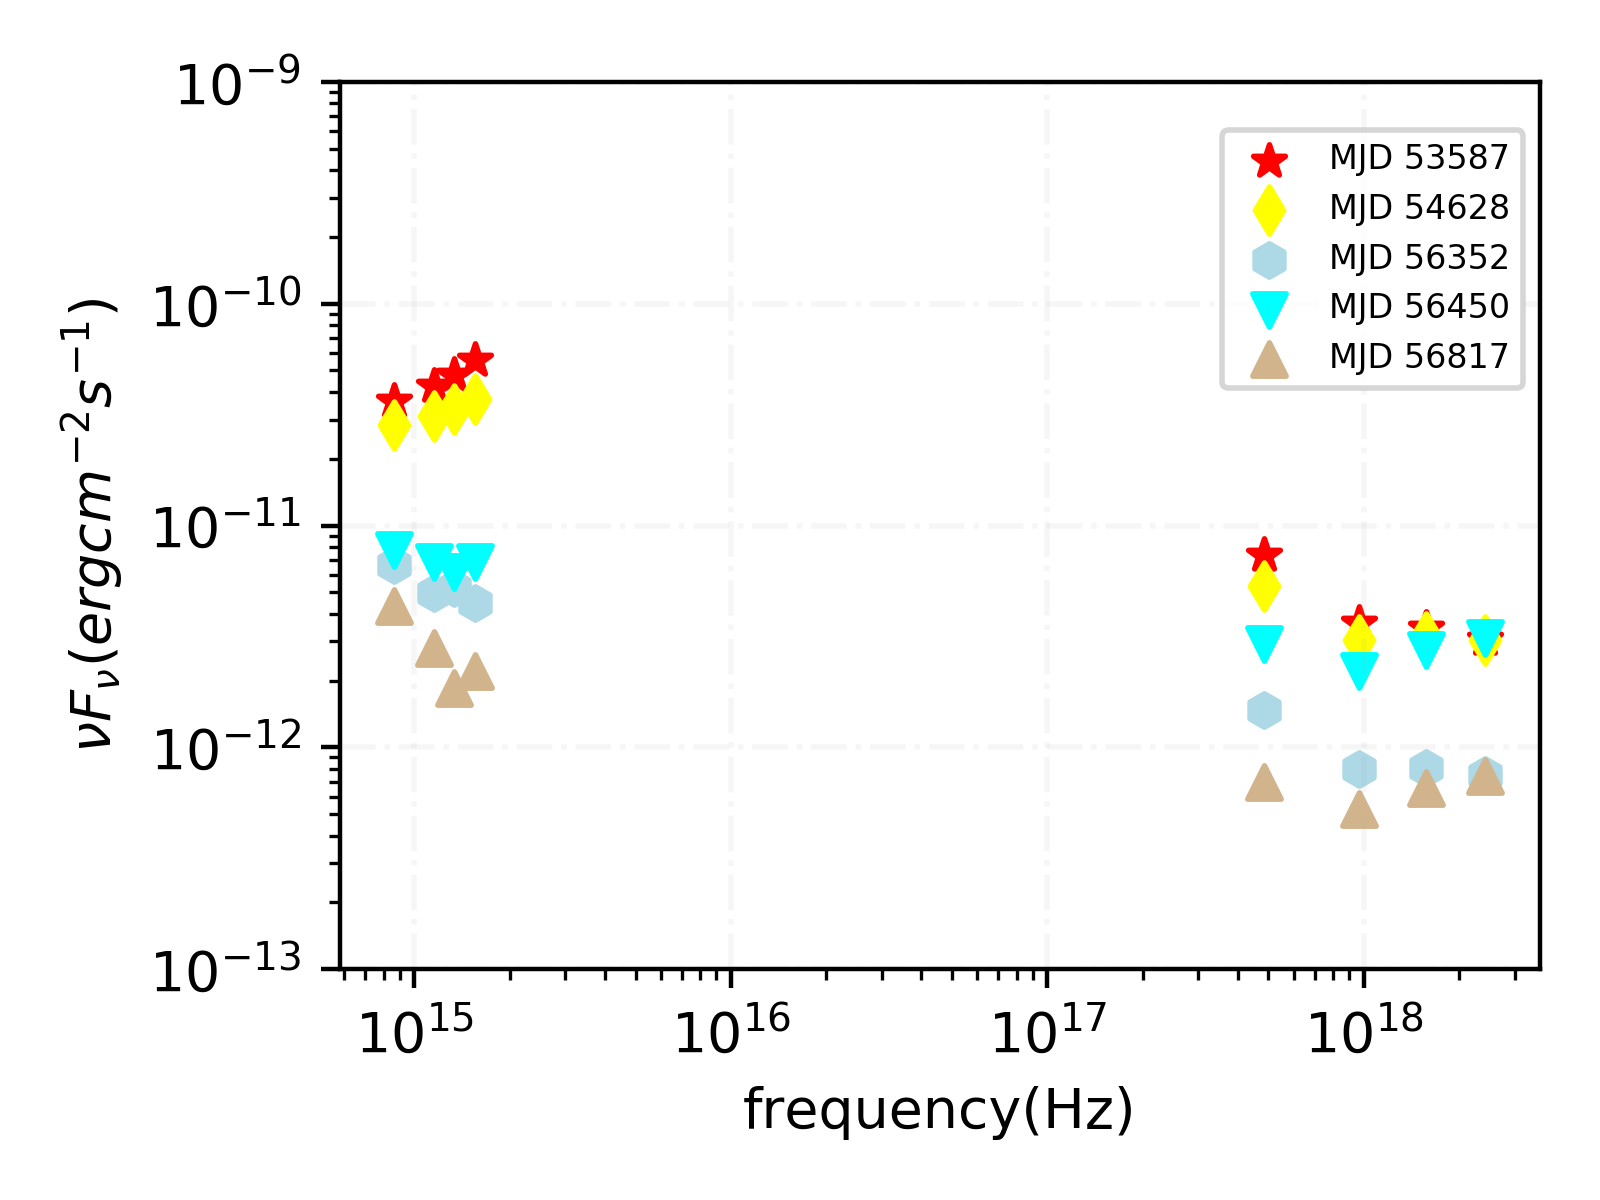
\includegraphics[width=0.9\textwidth]{./pic/Mrk1018_uvot_xray_sed.png}
    \caption{SED between X-ray and ultraviolet}
    \label{fig:xray-uvot-sed}
\end{figure}



\subsection{Correlation between X-ray and radio}\label{subsec:xray-radio}
We adopt data from intervals between X-ray and radio band as short as possible and find that correlation between the radio and X-ray flux is weak with a spearmanr coefficiency: -0.54, since the radio band flux of Mrk~1018 is almost flat relative to X-ray with a slope $\sim -0.1$ when fitting $log(L_{R})\propto log(L_{X-ray})$. 












\section{Discussion}\label{sec:discussion}




%It's also consistent with a conclusion in \citet{2018MNRAS.480.3898N}.  


\subsection{V-shape evolution}
During the fading period, the evolution of X-ray photn index and $\alpha_{OX}$ with flux represents anti-positive/positive correlation in two tracks(so called 'V-shape'). The V-shape both in $\Gamma-L_{2-10~keV}/L_{Edd}$ and $\alpha_{OX}-\lambda L_{2500\angstrom}/L_{Edd}$ diagram show much similarity with other changing-look AGNs \citep[see ][]{2019arXiv190904676R} and quasars \citep[see ][]{2019ApJ...883...76R}. Unfortunately, there is a distinct flux gap between two tracks for Mrk~1018 which could be caused by lack of observation during the transition period or two intrinsic states in Mrk~1018. The anti-positive correlation of $\Gamma-L_X/L_{Edd}$ in low-accreting AGNs is found with $10^{-10}\leq L_X/L_{Edd} \leq 10^{-3}$ and $10^{-6.5}\leq L_XL_{Edd} \leq 10^{-3}$, \citep[see][]{2014MNRAS.443...72J,2015MNRAS.447.1692Y}, respectively, while positive correlation of $\Gamma-L_X/L_{Edd}$ is found when $L_X/L_{Edd} \geq 10^{-3}$ \citep[see][]{2015MNRAS.447.1692Y}. X-ray binaries and AGNs share similar anti-positive/positive correlation between X-ray photon index and Eddington ratio below/above a critical value of $L_{\rm bol}/L_{\rm Edd}\sim 10^{-2}$ \citep[e.g.,][and references therein]{2008ApJ...682..212W,2009MNRAS.399..349G,2015MNRAS.447.1692Y}. The analogous of $\alpha_{OX}-L_{bol}/L_{Edd}$ in X-ray binaries and simulated AGNs spectral states compared to changing-look quasars are also found \citep[see ][]{2011MNRAS.417..280S,2011MNRAS.413.2259S,2019ApJ...883...76R}, which provides another link between stellar-mass black holes and super-massive black holes.


\subsection{Type transtion mechanism}
\citet{2014MNRAS.438.3340E} describes a evolutionary sequence that the AGN type evolution sequence:type 1 $\to$ 1.2/1.5 $\to$ 1.8/1.9 $\to$ 2 as luminosity (or accretion rate onto black hole) decreases in a disc-wind scenario for broad line region. It's consistent with the type evolution of Mrk~1018. The 2-10~keV flux variability reaches a factor around 8-10 between 2009 and 2016, which could be caused by the dimming of the central engine. The type transition timescale can be limited in $\sim 2$ years, while we find the variability timescale in two X-ray tracks can be as short as several months. 

While \citet{2008AJ....135.1505S} shows strong and positive $\Gamma-L_X$ correlation in 173 bright radio-quiet active galactic nuclei (AGNs) in the redshift range 0.1$\sim$4 when type I and no-type I AGNs are divided into sub-samples with luminosity range from $10^{42}$ to $10^{45} erg s^{-1}$, it seems that anti-positive/positive correlation between $\Gamma$ and X-ray luminosity or Eddington rate below/above the so-called critical accretion rate mainly relies on luminosity or accretion rate no matter what the type of AGNs are. As shown in Fig~\ref{fig:xrayappendgood-fandg-tmap} and ~\ref{fig:alpha_ox_luv}, we believe that $\alpha_{OX}-\lambda L_{2500\angstrom}/L_{Edd}$ relation is well linked to the types of AGNs, instead of $\Gamma-L_{X}$.    
 
%and references therein
%e.g.,
 

\begin{figure}
\centering
	% To include a figure from a file named example.*
	% Allowable file formats are eps or ps if compiling using latex
	% or pdf, png, jpg if compiling using pdflatex
	
\includegraphics[width=0.9\textwidth]{./pic/xrayappendgood-errorbar-f-g-tmap.png}
    \caption{$\Gamma$ and flux evolution of Mrk~1018. Blue arrows represent the rapid jump between left and right branches. Grey arrow represents the mini-outburst during 2016-2017.}
    \label{fig:xrayappendgood-fandg-tmap}
\end{figure}


\begin{figure}
\centering
	% To include a figure from a file named example.*
	% Allowable file formats are eps or ps if compiling using latex
	% or pdf, png, jpg if compiling using pdflatex
	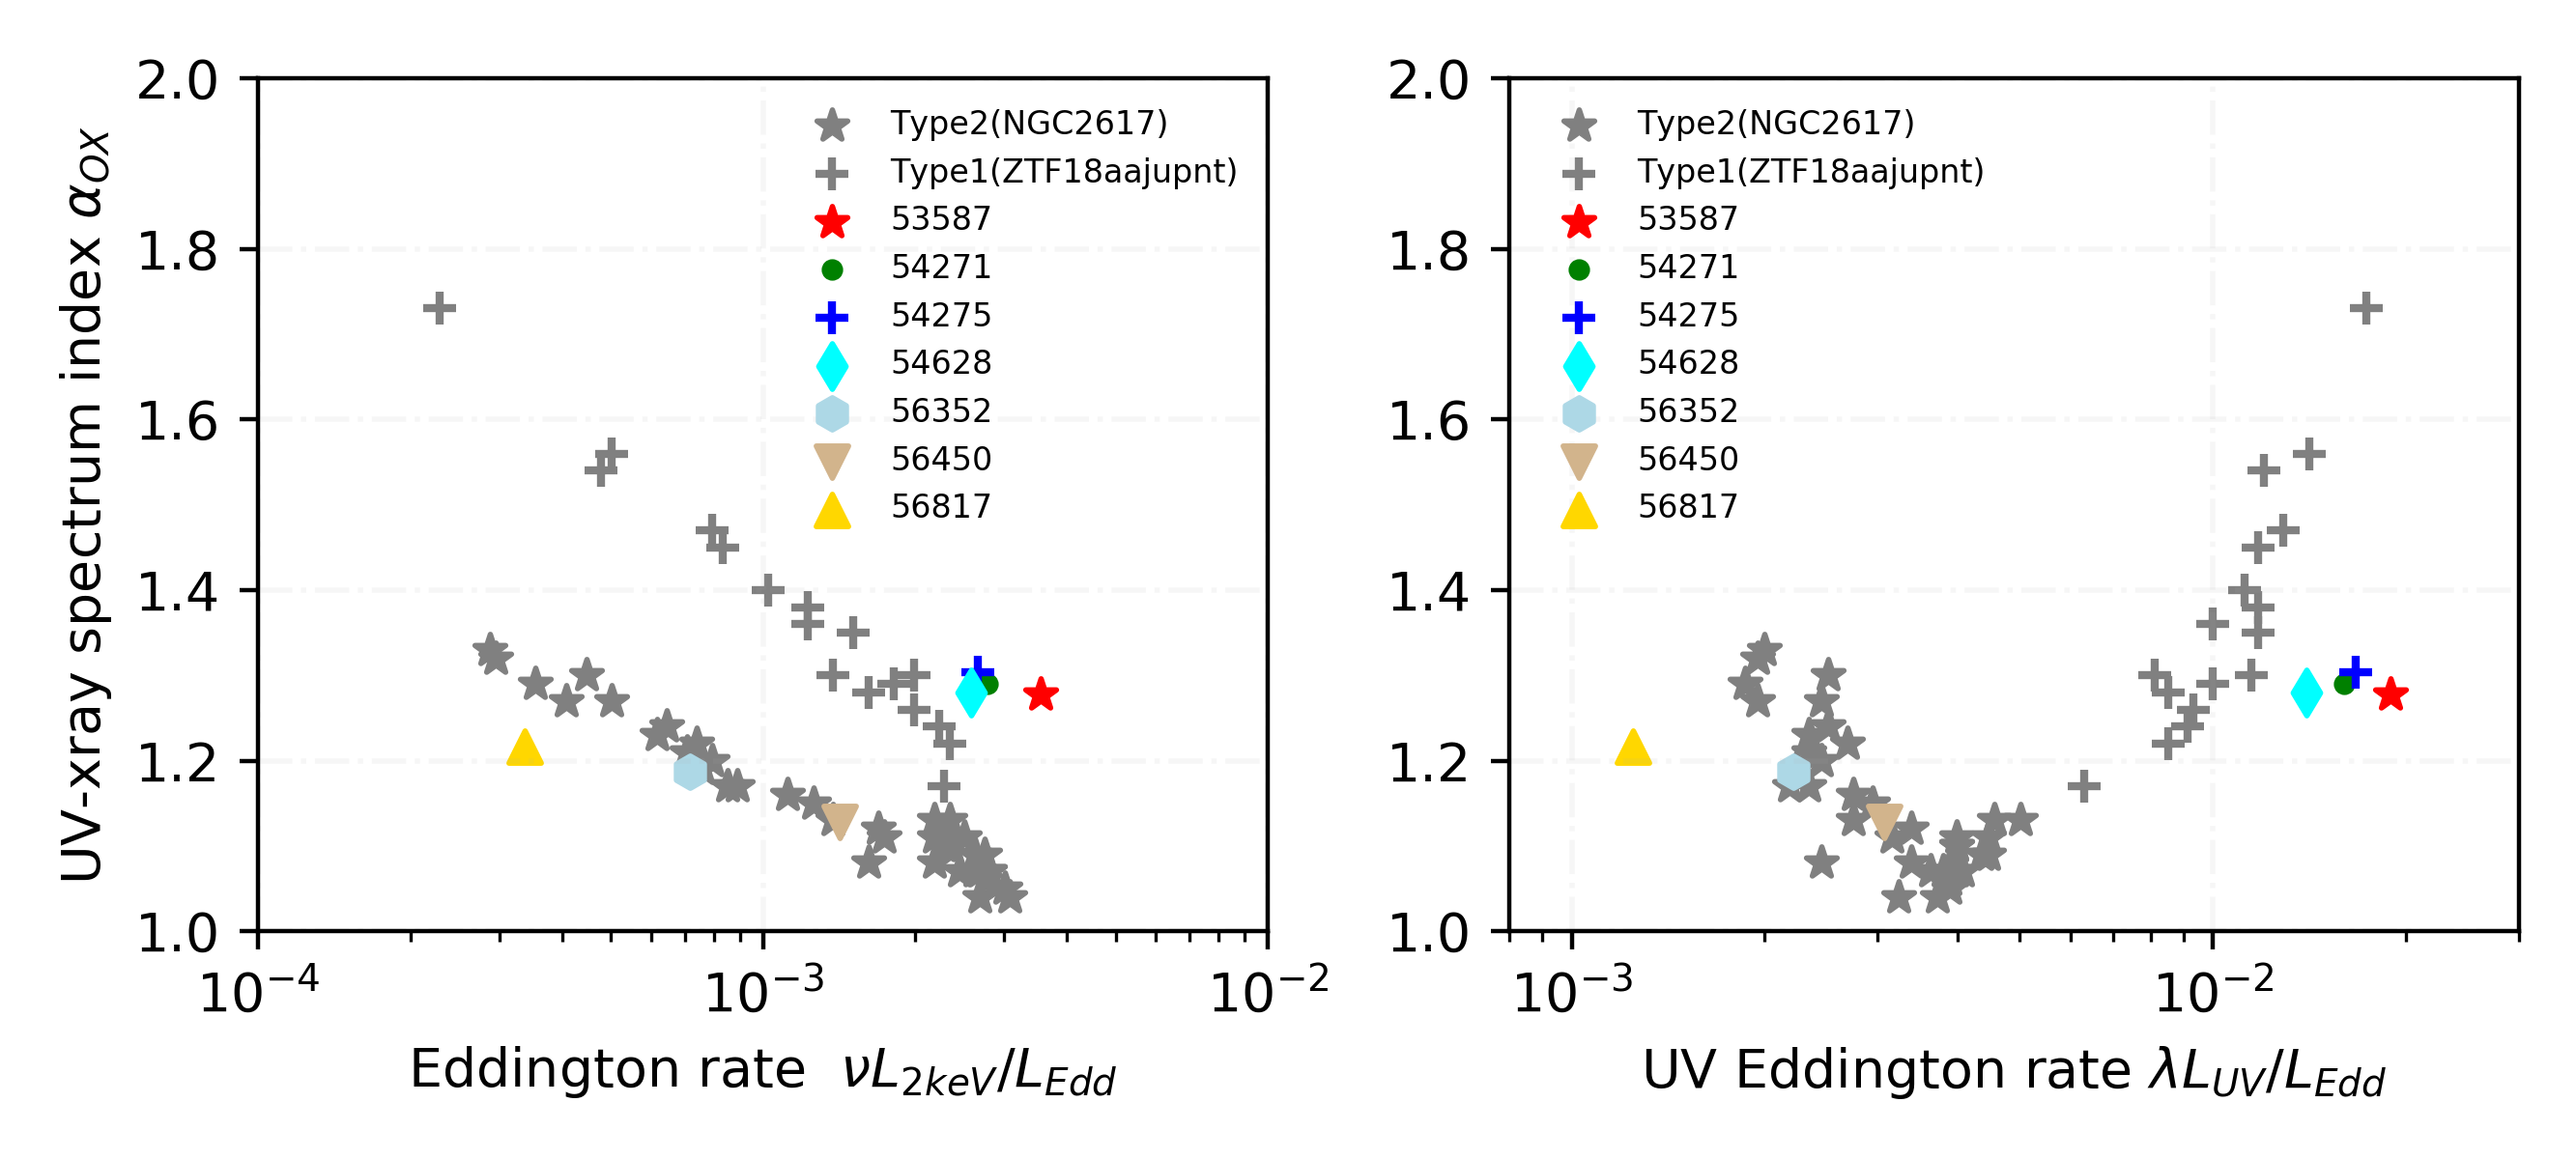
\includegraphics[width=0.9\textwidth]{./pic/Mrk1018_subplots_plus_2individuals_alpha_ox_L_x_Luv_rate.png}
    \caption{Mrk1018 and two other changing-look AGNs $\alpha_{OX}-\nu L_{2keV}/L_{Edd}$ and $\alpha_{OX}-\lambda L_{2500 \angstrom}/L_{Edd}$ diagram. Data of NGC~2617 and ZTF18aajupnt come from \citet{2019arXiv190904676R}.  }
    \label{fig:alpha_ox_luv}
\end{figure}


\subsection{Xray and ultraviolet }
We find a strong correlation between the optical and X-ray fluxes during the fading phase, which might correspond to near radiation region  between X-ray corona and accretion disk, as also suggested in \citet{2017A&A...607L...9K}. Within the long-term timescales(e.g., 6 years), the optical flux varies more than X-ray, while it is inverse during two re-brightening phases and type transition period.

%which may indicate that the optical emission is produced by re-processing of the X-rays in outer parts of the optically-thick wind coming from the accretion disk. 


\subsection{Spectrum shape and accretion rate}
From broad band SED from ultraviolet to X-ray, we can roughly estimate that the temperature of disk declines as the luminosity decreases.



\subsection{Radio and X-ray}
%Mrk~1018 is located nearly at the transition between two accretion mode, with relatively flat slope in radio and X-ray Eddington rate $\nu L_{\nu}/L_{Edd}-L_{2-10keV}/L_{Edd}$ diagram.
Mrk~1018 shows relatively flat radio-X-ray relation in the fundamental plane defined in \citet{2012MNRAS.419..267P}.

\begin{figure}
\centering
	% To include a figure from a file named example.*
	% Allowable file formats are eps or ps if compiling using latex
	% or pdf, png, jpg if compiling using pdflatex
	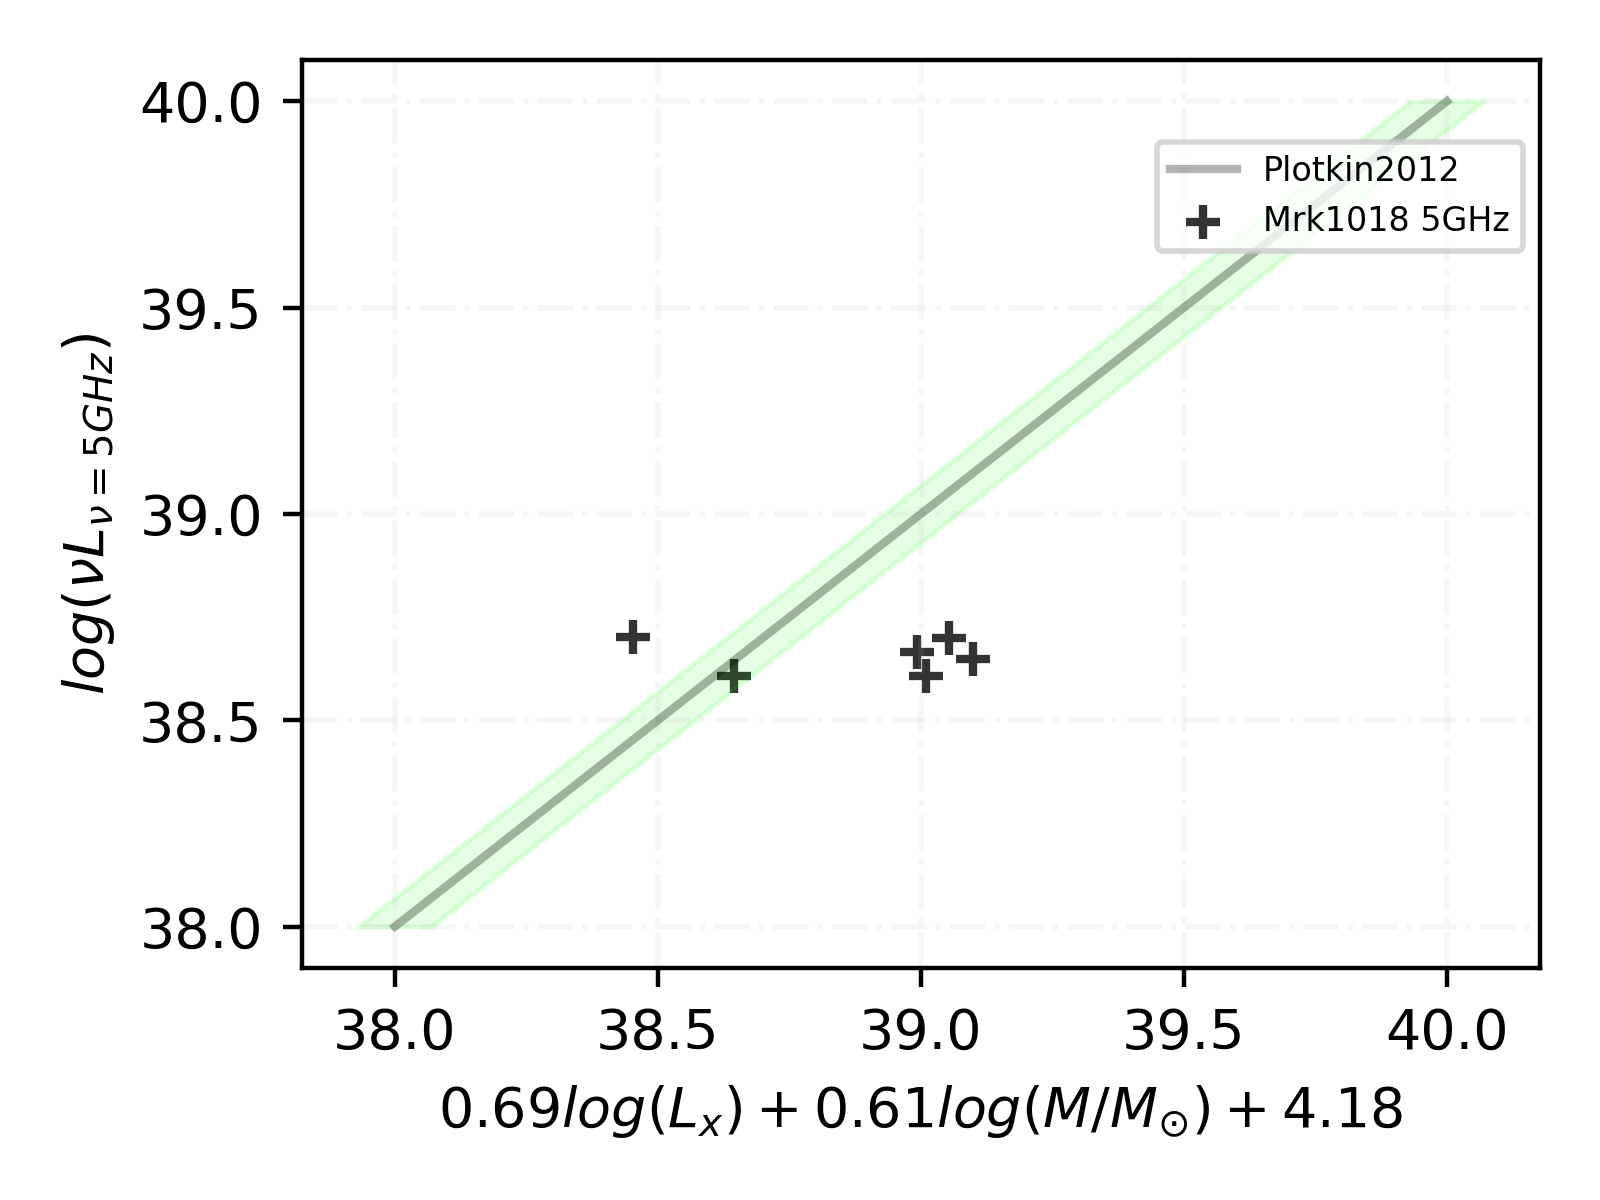
\includegraphics[width=0.9\textwidth]{./pic/Mrk1018_radio_xray_Plotkin2012.png}
    \caption{Mrk~1018's radio flux is flat relative to X-ray. Grey line shows the fundamental plane defined in \citet{2012MNRAS.419..267P} with intrinsic $\sigma=0.07$.}
    \label{fig:radio-xray-mass_relation_Plotkin2012}
\end{figure}


The severe variability of Mrk~1018 in short timescale provides a good target for intrinsic activity of individual Super-massive Black Holes(SMBH). Considering all observational evidence, we can draw a full picture about how Mrk~1018's spectrum evolves with luminosity. As the luminosity declines, both corona and accretion disk varies.  



\acknowledgments

We thank Linhui Wu for disscussion on the VLA data reduction. This work is supported by...

%% To help institutions obtain information on the effectiveness of their 
%% telescopes the AAS Journals has created a group of keywords for telescope 
%% facilities.
%
%% Following the acknowledgments section, use the following syntax and the
%% \facility{} or \facilities{} macros to list the keywords of facilities used 
%% in the research for the paper.  Each keyword is check against the master 
%% list during copy editing.  Individual instruments can be provided in 
%% parentheses, after the keyword, but they are not verified.


\vspace{5mm}
\facilities{\chandra, \swift(XRT and UVOT), \xmm, \nustar,
VLA}

%% Similar to \facility{}, there is the optional \software command to allow 
%% authors a place to specify which programs were used during the creation of 
%% the manusscript. Authors should list each code and include either a
%% citation or url to the code inside ()s when available.

\software{HEASOFT(v6.26),
          SAS (v16.1.0),
          CIAO (v4.10), CASA(v5.3.0),
          Astropy \citep{2013A&A...558A..33A}
          }

%% Appendix material should be preceded with a single \appendix command.
%% There should be a \section command for each appendix. Mark appendix
%% subsections with the same markup you use in the main body of the paper.

%% Each Appendix (indicated with \section) will be lettered A, B, C, etc.
%% The equation counter will reset when it encounters the \appendix
%% command and will number appendix equations (A1), (A2), etc. The
%% Figure and Table counter will not reset.

\clearpage
%\bibliographystyle{mnras}
\bibliography{refMrk1018}{}
% if your bibtex file is called example.bib
\bibliographystyle{aasjournal}
\clearpage

\begin{table}
\centering
\caption{{ \bf X-ray fit parameters of Mrk~1018. } Columns include the date of the observation, the facility, observation id, reduced $\chi ^2$ of the best fit model, the photon index $\Gamma$ with 90\% uncertainty, and the flux in 2-10~keV after Galactic-absorption correction. }
\label{tab:table1}

\begin{tabular}{lcccccc}
\hline
\hline
 
  Date   &   Instrument & obsid  & $\chi ^2$  &$\Gamma$  &  $F_{2-10keV}$  & \\ 
  (MJD)  &              &        &          &                    &  [erg cm$^{-2}$ s$^{-1}$] &      
 \\  \hline
53385 & X & 201090201 & 0.98 & 1.73 $\pm$ 0.07 & 9.7e-12 $\pm$ 6e-13 \\ 
53587 & S & 35166001 & 0.78 & 1.93 $\pm$ 0.1 & 1.15e-11 $\pm$ 6.99e-13 \\ 
54271 & S & 30955001 & 1.01 & 1.89 $\pm$ 0.09 & 9.39e-12 $\pm$ 4.47e-13 \\ 
54274 & S & 30955002 & 1.07 & 1.91 $\pm$ 0.08 & 8.54e-12 $\pm$ 4e-13 \\ 
54276 & S & 30955003 & 1.02 & 1.96 $\pm$ 0.08 & 8.38e-12 $\pm$ 3.47e-13 \\ 
54628 & S & 35776001 & 1.19 & 1.75 $\pm$ 0.07 & 9.98e-12 $\pm$ 3.96e-13 \\ 
54685 & X & 554920301 & 1.16 & 1.79 $\pm$ 0.02 & 1.13e-11 $\pm$ 2e-13 \\ 
55527$^{(a)}$ & C & 12868 & 1.1 & 1.7 $\pm$ 0.03 & 9.26e-12 $\pm$ 1.9e-13 \\ 
56353 & S & 49654001 & 1.42 & 1.82 $\pm$ 0.38 & 2.59e-12 $\pm$ 5.52e-13 \\ 
56450 & S & 49654002 & 1.23 & 1.38 $\pm$ 0.19 & 7.9e-12 $\pm$ 8.21e-13 \\ 
56818 & S & 49654004 & 0.75 & 1.38 $\pm$ 0.31 & 1.88e-12 $\pm$ 3.37e-13 \\ 
57428 & N & 60160087002 & 1.23 & 1.85 $\pm$ 0.08 & 1.8e-12 $\pm$ 1e-13 \\ 
57429 & S & 80898001 & 0.96 & 1.72 $\pm$ 0.2 & 1.61e-12 $\pm$ 1.89e-13 \\ 
57434 & S & 80898002 & 0.9 & 1.45 $\pm$ 0.2 & 2.17e-12 $\pm$ 2.77e-13 \\ 
57443 & C & 18789 & 0.82 & 1.7 $\pm$ 0.03 & 1.3e-12 $\pm$ 3e-14 \\ 
57801 & C & 19560 & 1.26 & 1.61 $\pm$ 0.02 & 2.48e-12 $\pm$ 4e-14 \\ 
58123 & N & 60301022002 & 1.34 & 1.8 $\pm$ 0.06 & 2.1e-12 $\pm$ 1e-13 \\ 
58125 & S & 88207001 & 1.04 & 1.63 $\pm$ 0.25 & 2.02e-12 $\pm$ 3.08e-13 \\ 
58126 & C & 20366 & 1.05 & 1.6 $\pm$ 0.03 & 1.84e-12 $\pm$ 5e-14 \\ 
58180 & C & 20367 & 1.02 & 1.61 $\pm$ 0.04 & 1.59e-12 $\pm$ 5e-14 \\ 
58182 & N & 60301022003 & 1.03 & 1.8 $\pm$ 0.06 & 1.5e-12 $\pm$ 7e-14 \\ 
58281 & C & 20368 & 1.02 & 1.62 $\pm$ 0.03 & 1.77e-12 $\pm$ 5e-14 \\ 
58316 & N & 60301022005 & 0.85 & 1.74 $\pm$ 0.05 & 2e-12 $\pm$ 9e-14 \\ 
58317 & S & 88207003 & 1.01 & 1.61 $\pm$ 0.23 & 2.18e-12 $\pm$ 3.12e-13 \\  \\ \hline
\end{tabular}\\
Notes: Here the superscripts $^{(a)}$ represents fit result that are taken from \citet{2017A&A...607L...9K}. Instrument indicate by C-\chandra, S-\swift, X-\xmm, N-\nustar. 
\end{table}







\begin{table}
\centering
\caption{{\bf $\alpha_{ox}$ of Mrk~1018 with simultaneous XRT and UVOT observation.} Columns include the date of the observation, $\alpha_{ox}$, flux in 2-10~keV, $\nu F_{uw1}$, and Eddington rate.}
\label{tab:tablealpha_ox}
\begin{tabular}{lcccccc}
\hline
\hline
 
 Date &   $\alpha_{ox}$  & $F_{2-10keV}$  &$\nu F_{uw1}$  & $L_{2-10keV}/L_{Edd}$ &   $\nu L_{uw1}/L_{Edd}$  \\ 
 (MJD)&                   &   [erg cm$^{-2}$ s$^{-1}$]   &[erg cm$^{-2}$ s$^{-1}$]    &                    &            
 \\ \hline
53587 & 1.29 & 1.14e-11 & 3.92e-11 & 5.53e-03 & 1.90e-02 \\ 
54271 & 1.30 & 9.34e-12 & 3.31e-11 & 4.51e-03 & 1.60e-02 \\ 
54275 & 1.31 & 8.78e-12 & 3.45e-11 & 4.24e-03 & 1.67e-02 \\ 
54628 & 1.29 & 9.85e-12 & 2.89e-11 & 4.76e-03 & 1.40e-02 \\ 
56352 & 1.20 & 2.59e-12 & 4.58e-12 & 1.25e-03 & 2.22e-03 \\ 
56450 & 1.14 & 8.26e-12 & 6.35e-12 & 3.99e-03 & 3.07e-03 \\ 
56817 & 1.23 & 1.98e-12 & 2.58e-12 & 9.57e-04 & 1.25e-03 \\ \hline
\end{tabular}   
\end{table}
\begin{table}
\centering
\caption{{\bf VLA observation of Mrk~1018.} Columns include the date of observation, project name, band, frequency, integrated flux, radio spectral index ($\alpha$) and reference.}
\label{tab:tableradio}
\begin{tabular}{lcccccr}
\hline
\hline
 
 Date &  project & band  & Frequency  &$F_{int}$   & $\alpha$ & Reference  \\ 
 (MJD)&         &        &   [GHz]   &[mJy]     &                &         \\ \hline
    \multirow{2}*{46032} & \multirow{2}*{AU0020} & L    & 1.49  & 4.21  $\pm$ 0.23  & \multirow{2}*{0.52 $\pm0.07$} &\\
    \,          &        & C     & 4.86  & 2.29  $\pm$ 0.14  & & \\
    47261     & AB0476 & C     & 4.86  & 1.91  $\pm$ 0.23  &  &\\
    47692     & AB0540A & C     & 4.86  & 2.62  $\pm$ 0.16  &  &\\
    47732     & AB0540B & C     & 4.86  & 2.31  $\pm$ 0.17  & & \\
    49820.5 $\pm$ 773.5 & AB0628 & L     & 1.4   & 4.20  $\pm$ 0.45  &  & \citet{1998AJ....115.1693C} \\
    49820.5 $\pm$ 773.5 & AB0628 & L     & 1.4   & 4.15  $\pm$ 0.25  &  & \citet{1997ApJ...475..479W} \\
    50219.5 $\pm$ 1078.5 & AB0308 & L     & 1.4   & 4.20  $\pm$ 0.54  &  & \citet{2002AJ....124..675C}\\
    50970     & AB0878 & X     & 8.46  & 2.47  $\pm$ 0.17  & 0.3 $\pm0.08$\\
    52246.5 $\pm$ 278.5 & AB0950 & L     & 1.4   & 4.15  $\pm$ 0.25  & & \citet{2003yCat.8071....0B} \\
    54872.5 $\pm$ 51.5  & AR685 & L     & 1.4   & 3.69  $\pm$ 0.19  &  & \citet{2011AJ....142....3H}\\
    54878   & AB1314 & L     & 1.4   & 3.36  $\pm$ 0.20  &  & \citet{2012yCat.8090....0B} \\
    56550 $\pm$ 8     & 13B-272 & L     & 1.4   & 3.85  $\pm$ 0.31  &  & \citet{2016MNRAS.460.4433H} \\

    \multirow{3}*{57481}     &  \multirow{3}*{16A-444} & C     & 5     & 2.56  $\pm$ 0.13  & \multirow{3}*{0.02$\pm0.05$}& \\
              &     & X     & 10    & 2.16  $\pm$ 0.11  & &\\
              &    &  K     & 22    & 2.46  $\pm$ 0.12  &  &\\
    57719     & 16B-084 & X     & 10    & 1.78  $\pm$ 0.09  &   &\\

    57731     & 16B-084 & X     & 10    & 1.97  $\pm$ 0.10  &  &\\

    57768     & 16B-084 & C     & 5     & 2.07  $\pm$ 0.10  & 0 &\\
    58087     & VLASS1.1 & L     & 3     & 2.30  $\pm$ 0.36  & & \\
    
    58472     & 18B-245 & K     & 20    & 2.71  $\pm$ 0.14  &  & \\



\hline 
\end{tabular}   
\end{table}




     
\begin{table}
\centering
\caption{{\bf Radio and X-ray luminosity diagram.} Columns include the date of the radio observation, the radio spectrum index $\alpha_{radio}$, the date of X-ray observation, the interval between two bands, the flux and luminosity rescaled to 4.8 and 8.4~GHz, the X-ray flux and luminosity in 2-10~keV band.}
\label{tab:table4}
\begin{tabular}{lllllllllr}
\hline
\hline

$T_{Radio}$ &  $\alpha_{Radio}$ & $T_{X-ray}$ & $\delta$ T & $F_{2-10keV}$ & $F_{4.8GHz}$ & $F_{8.4GHz}$ &  $\nu L_{\nu=4.8GHz}$ &  $\nu L_{\nu=8.4GHz}$ & $L_{\rm{2--10~keV}}$ \\ 
(MJD)  &  & (MJD)  &(day)  &[erg$~s^{-1}~\rm{cm}^{-2}$] & [mJy)& (mJy)]& [erg$~s^{-1} $] & [erg$~s^{-1} $]& [erg$~s^{-1} $]\\
\hline

52246.5 & 0.42 & 53385 & 1138 & 9.70e-12 & 2.47 & 1.96 & 5.00e38 & 6.92e38 & 4.09e43 \\ 
54318 & 0.42 & 54276 & 42 & 8.78e-12 & 2.00 & 1.58 & 4.05e38 & 5.60e38 & 3.70e43 \\ 
54872.5 & 0.42 & 54685 & 188 & 1.13e-11 & 2.20 & 1.74 & 4.45e39 & 6.15e39 & 4.76e44 \\ 
56550 & 0.42 & 56450 & 100 & 8.26e-12 & 2.29 & 1.81 & 4.64e40 & 6.42e40 & 3.48e45 \\ 
57481 & 0.17 & 57443 & 38 & 1.30e-12 & 2.49 & 2.27 & 5.04e41 & 8.02e41 & 5.48e45 \\ 
57768 & 0.17 & 57801 & 33 & 2.48e-12 & 2.00 & 1.82 & 4.05e42 & 6.45e42 & 1.04e47 \\  \hline
\end{tabular}\\
Notes: We assume the $\alpha_{Radio}$ before/after the type transition as a constant, respectively. 
\end{table}


%\appendix
%\section{Appendix}


%\clearpage


%\clearpage


%% For this sample we use BibTeX plus aasjournals.bst to generate the
%% the bibliography. The sample63.bib file was populated from ADS. To
%% get the citations to show in the compiled file do the following:
%%
%% pdflatex sample63.tex
%% bibtext sample63
%% pdflatex sample63.tex
%% pdflatex sample63.tex




%% This command is needed to show the entire author+affiliation list when
%% the collaboration and author truncation commands are used.  It has to
%% go at the end of the manuscript.
%\allauthors

%% Include this line if you are using the \added, \replaced, \deleted
%% commands to see a summary list of all changes at the end of the article.
%\listofchanges
% Don't change these lines
%\bsp	% typesetting comment
%\label{lastpage}
\end{document}

% End of file `sample63.tex'.
